% To be \input{}'ed from the various subfolders - do not attempt to compile on
% its own!

\documentclass[10pt]{beamer}
\usepackage[T1]{fontenc}
\usepackage[utf8]{inputenc}

\graphicspath{{}{figures/}{screenshots/}}

\usetheme[progressbar=frametitle]{metropolis}
\usepackage{appendixnumberbeamer}

\usepackage{booktabs}
\usepackage[scale=2]{ccicons}

\usepackage{pgfplots}
\pgfplotsset{compat=1.12}
\usepgfplotslibrary{dateplot}

\usetikzlibrary{calc,fit,patterns}
\usepackage[absolute,overlay]{textpos}

\usepackage{xspace}
\newcommand{\themename}{\textbf{\textsc{metropolis}}\xspace}

\newcommand*{\file}[1]{\texttt{#1}}

\usepackage{xcolor}
\usepackage{listings}
\lstset{columns=fullflexible}
\lstdefinelanguage{EOL}{
morekeywords={delete,import,for,while,in,and,or,self,operation,return,def,var,throw,if,new,else,transaction,abort,
break,breakAll,continue,assert,assertError,not, switch, case, default},
sensitive=true,
morecomment=[l]{//},
morecomment=[l]{--},
morecomment=[s]{/*}{*/},
morecomment=[s]{-*}{*-},
morestring=[b]",
morestring=[b]',
showstringspaces=false
}

\lstnewenvironment{java}{\lstset{language=Java,
		frame=tb,
        tabsize=3,
        morekeywords={implies, in, result},
        basicstyle=\footnotesize,
        keywordstyle=\bfseries,
        ndkeywordstyle=\bfseries,
        commentstyle=\itshape,
		morecomment=[l]{--},
        stringstyle=\ttfamily,
		showspaces=false,
        flexiblecolumns,
        literate={->}{$\to$}{2} {--}{-$\,$-}{2} {<=}{$\le$}{2} {>=}{$\ge$}{2} {<>}{$<\,>$}{3},
        sensitive, extendedchars, texcl}}{}

\lstnewenvironment{ocl}{\lstset{language=[decorative]OCL,
	frame=tb,
	tabsize=3,
	morekeywords={implies,result,flatten,body,init,OrderedSet,Tuple,TupleType,def,attr,oclIsUndefined,oclIsInvalid,OclState,let,in},
	basicstyle=\footnotesize,
	keywordstyle=\bfseries,
	ndkeywordstyle=\bfseries,
	commentstyle=\itshape,
	stringstyle=\ttfamily,
	showspaces=false,
	flexiblecolumns,
	literate={->}{$\to$}{2} {--}{-$\,$-}{2} {<=}{$\le$}{2} {>=}{$\ge$}{2} {<>}{$<\,>$}{3},
	sensitive, extendedchars, texcl}}{}


\lstdefinelanguage{gremlin}{
morekeywords={as,def,fill,filter,groupCount,has,idx,inE,inV,is,label,length,match,outE,outV,v,values},
sensitive=true,
morecomment=[l]{//}
}

% "page cs" coordinate system
% From http://tex.stackexchange.com/questions/89588/
%
% Defining a new coordinate system for the page:
%
% --------------------------
% |(-1,1)    (0,1)    (1,1)|
% |                        |
% |(-1,0)    (0,0)    (1,0)|
% |                        |
% |(-1,-1)   (0,-1)  (1,-1)|
% --------------------------
\makeatletter
\def\parsecomma#1,#2\endparsecomma{\def\page@x{#1}\def\page@y{#2}}
\tikzdeclarecoordinatesystem{page}{
    \parsecomma#1\endparsecomma
    \pgfpointanchor{current page}{north east}
    % Save the upper right corner
    \pgf@xc=\pgf@x%
    \pgf@yc=\pgf@y%
    % save the lower left corner
    \pgfpointanchor{current page}{south west}
    \pgf@xb=\pgf@x%
    \pgf@yb=\pgf@y%
    % Transform to the correct placement
    \pgfmathparse{(\pgf@xc-\pgf@xb)/2.*\page@x+(\pgf@xc+\pgf@xb)/2.}
    \expandafter\pgf@x\expandafter=\pgfmathresult pt
    \pgfmathparse{(\pgf@yc-\pgf@yb)/2.*\page@y+(\pgf@yc+\pgf@yb)/2.}
    \expandafter\pgf@y\expandafter=\pgfmathresult pt
}
\makeatother
% Draws a grid for easier referencing of page cs values
\newcommand{\printtikzpagegrid}{
  \tiny
  \begin{tikzpicture}[overlay,remember picture,every node/.style={inner sep=.1em,draw=black!20,fill=white}]
    \foreach \x in {0,...,9} {
      \foreach \y in {0,...,9} {
        \node at (page cs:0.\x,0.\y) {};
        \node at (page cs:0.\x,-0.\y) {};
        \node at (page cs:-0.\x,0.\y) {};
        \node at (page cs:-0.\x,-0.\y) {};
      }
    }
    \node at (page cs:0,0) {0,0};
    \node at (page cs:0.5,0.5) {.5,.5};
    \node at (page cs:0.5,-0.5) {.5,-.5};
    \node at (page cs:-0.5,0.5) {-.5,.5};
    \node at (page cs:-0.5,-0.5) {-.5,-.5};
    \node at (page cs:1,1) {1,1};
    \node at (page cs:1,-1) {1,-1};
    \node at (page cs:-1,1) {-1,1};
    \node at (page cs:-1,-1) {-1,-1};
  \end{tikzpicture}
  \normalsize
}

\title{Taming Large Models\\with Hawk and NeoEMF}
%\subtitle{A modern beamer theme}
\date{MoDELS'2018, 14--19 October 2018}
\author{A. García-Domínguez, D. S. Kolovos, K. Barmpis, G. Daniel, G. Sunyé}
%\institute{Center for modern beamer themes}
% \titlegraphic{\hfill\includegraphics[height=1.5cm]{logo.pdf}}


\begin{document}

\maketitle

\pgfset{/metropolis/inner/sectionpage/.cd, none}
\section{Introduction}
\section{Hawk}

\pgfset{/metropolis/inner/sectionpage/.cd, progressbar}
\section{NeoEMF}

\begin{frame}[t]\frametitle{NeoEMF: Architecture}
  \begin{center}
    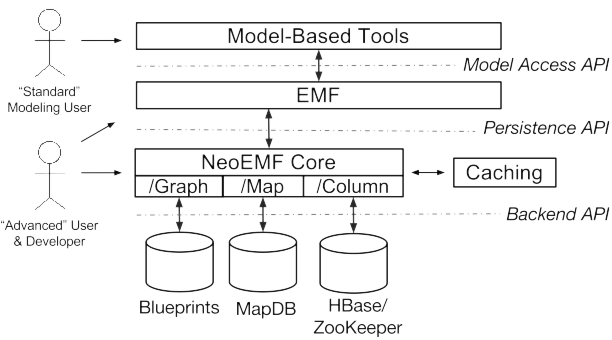
\includegraphics[width=\textwidth]{neoemf-architecture.png}
  \end{center}
\end{frame}

\begin{frame}[t]\frametitle{NeoEMF: project website}
  \begin{center}
    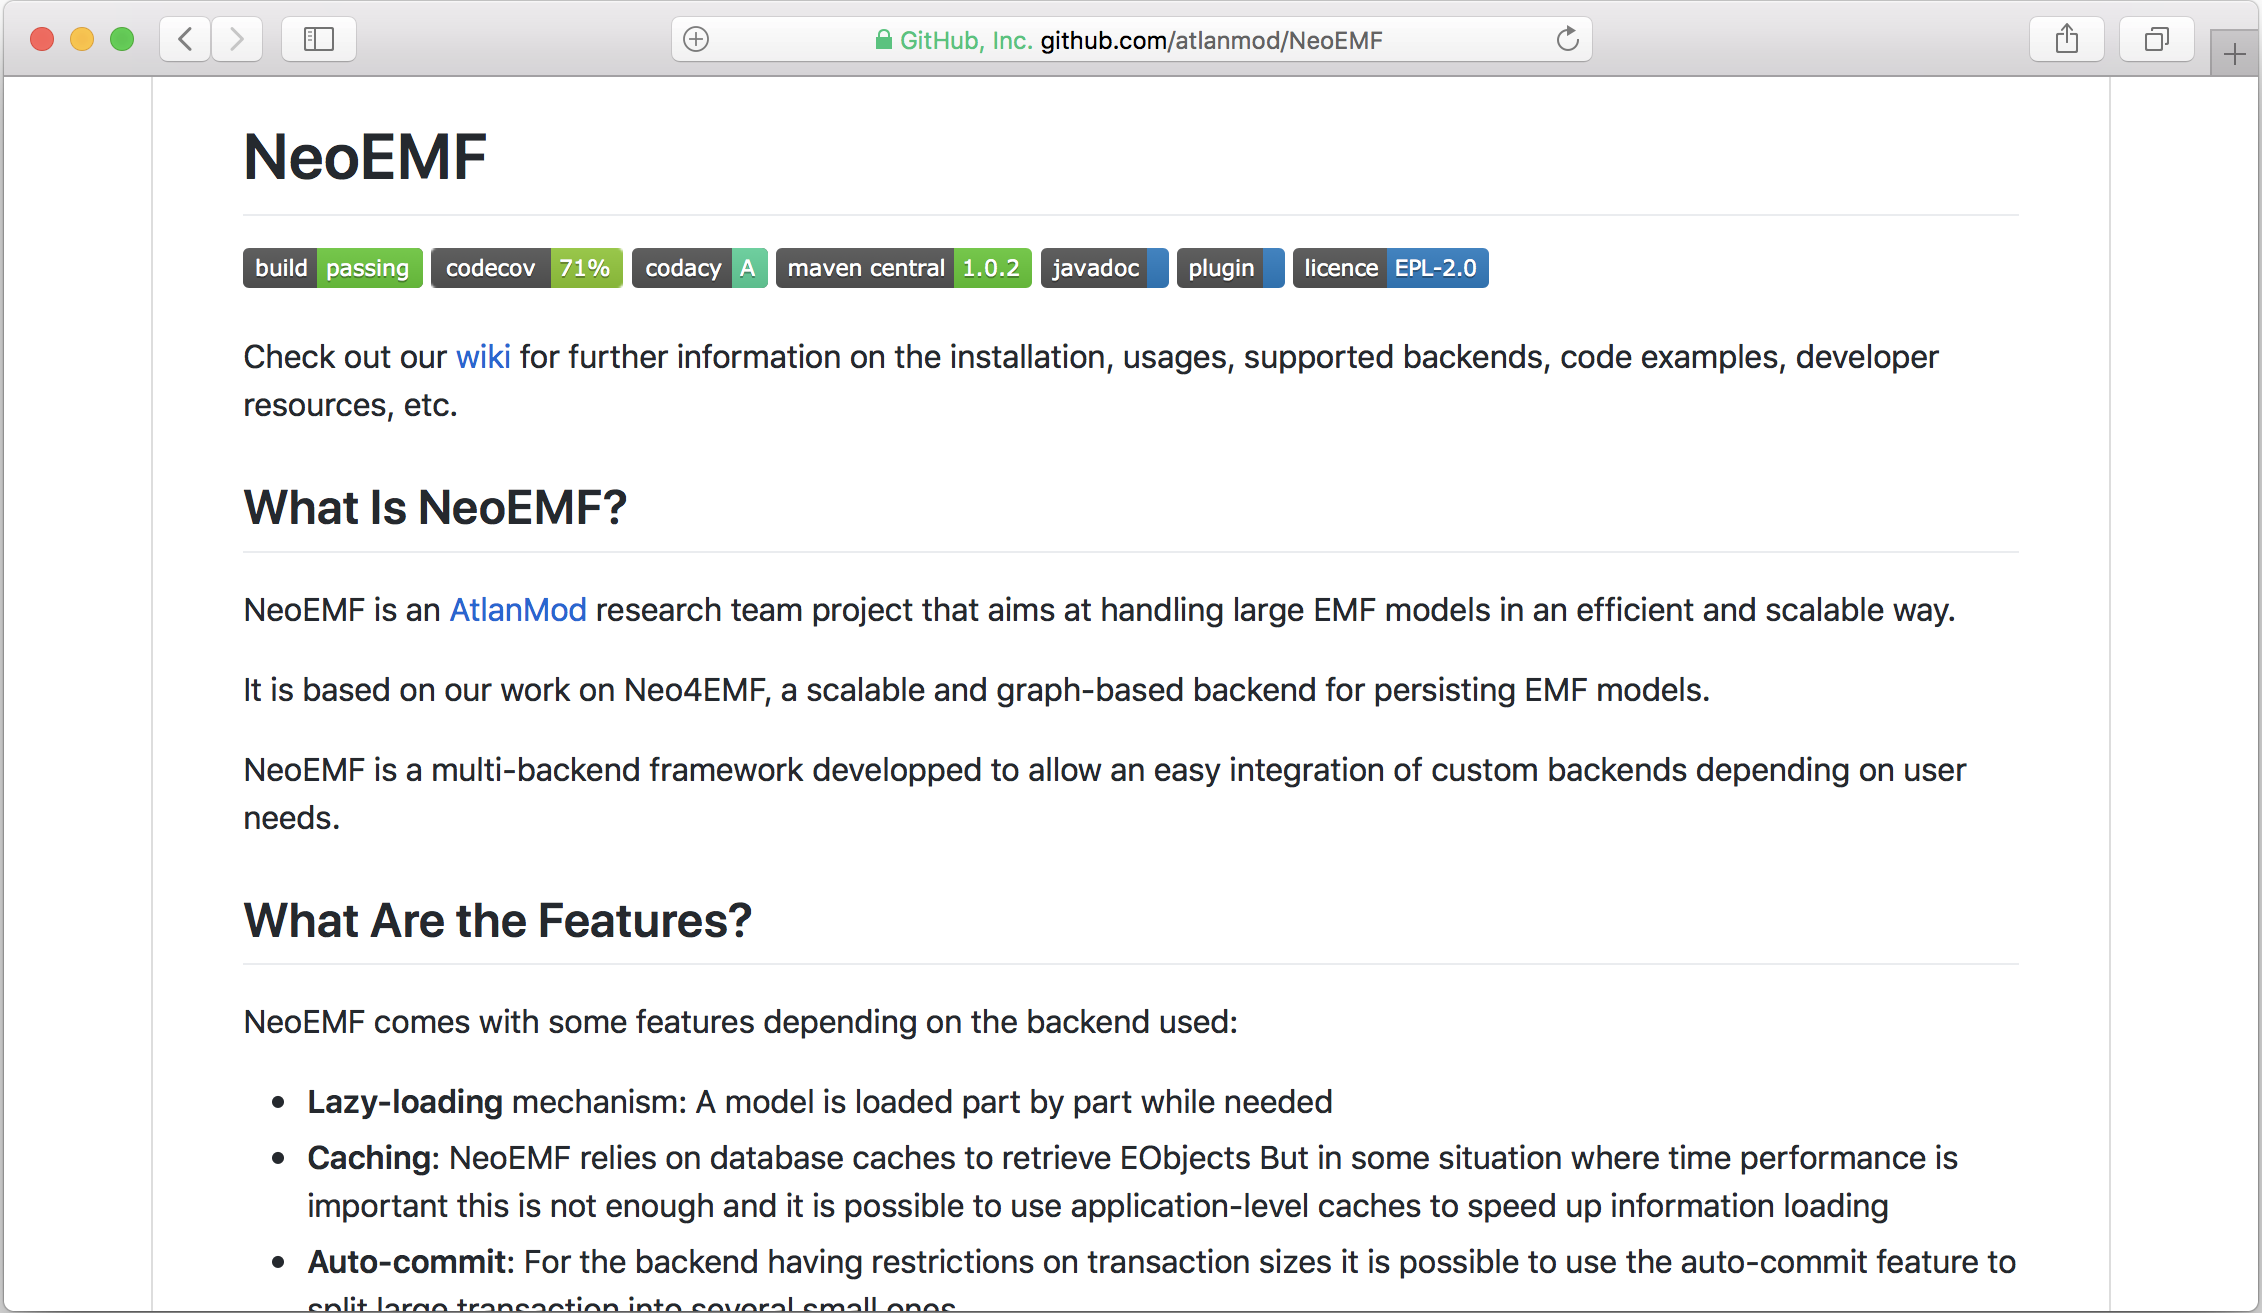
\includegraphics[width=\textwidth]{neoemf-github.png}
  \end{center}
	
  \begin{itemize}
  \item \url{https://github.com/atlanmod/NeoEMF}
  \item Open source project under the Eclipse Public License 2.0
  \end{itemize}
\end{frame}

\begin{frame}[c]\frametitle{NeoEMF Datastores~\cite{DBLP:conf/models/DanielSBTVGC16}}
	\begin{itemize}
	\item NeoEMF/Graph
		\begin{itemize}
		\item Efficient model traversal using rich query language
		\item Mogwaï framework (OCL to Gremlin translation)
		\end{itemize}
	\item NeoEMF/Map
		\begin{itemize}
		\item Fast access to atomic operations
		\item Designed for EMF-API calls
		\end{itemize}
	\item NeoEMF/Column
		\begin{itemize}
		\item Transparent model distribution
		\item Concurrent read/write
		\item Distributed model transformations (ATL-MR)
		\end{itemize}
	\end{itemize}
\end{frame}

\begin{frame}[c]\frametitle{NeoEMF Key Features}
	\begin{itemize}
	\item Lazy-loading
	\item Compliant with EMF API
	\item Easy to integrate in existing applications
	\item EMF-Compatible code generation
	\item Advanced caching (+ prefetching) strategies
	\item Efficient XMI importer
	\end{itemize}
\end{frame}

\begin{frame}[fragile]\frametitle{Initialise a New Resource}
	\begin{enumerate}
	\item Create a new URI to locate a file-based resource.
	\item Create the resource.
	\end{enumerate}
	
  \begin{java}
    URI uri = MyUriBuilder.builder().fromFile(new File("<db_path>"));

    ResourceSet resourceSet = new ResourceSetImpl();
    Resource resource = resourceSet.createResource(uri);
  \end{java}
\end{frame}

\begin{frame}[fragile]\frametitle{Save/Load Resource}
	
	\begin{enumerate}
	\item Create a new configuration builder.
	\item Save and unload resource.
	\end{enumerate}
  \begin{java}
    ImmutableConfig config = MyConfig.newConfig()
    .autoSave(50000)              
    .log()                        
    .withOption("key", "value");  

    resource.load(config.asMap()); 

    // Do something on the resource

    resource.save(config.asMap()); 
    resource.unload();
  \end{java}
	
\end{frame}

\begin{frame}[fragile]\frametitle{Modify existing resource}
	\begin{enumerate}
	\item Load resource.
	\item Modify contents.
	\item Save resource. 
	\end{enumerate}
	
  \begin{java}
    ImmutableConfig config = MyConfig.newConfig()
    .cacheContainers()
    .cacheMetaclasses();

    URI uri = MyUriBuilder.builder().fromFile(new File("db_path"));

    Resource resource = new ResourceSetImpl().createResource(uri);
    resource.load(config.asMap());

    MyClass myClass = (MyClass) resource.getContents().get(0);
    myClass.setName("NewName");

    resource.save(config.asMap());
    resource.unload();
  \end{java}
\end{frame}

\begin{frame}[standout]
  Demo time!

  Let's import a Java model, save it in Neo4j and query the database.
\end{frame}

\begin{frame}[c]\frametitle{Discussion}
	\begin{itemize}
	\item Graph databases outperform relational ones for several navigation steps queries.
	\item But model loading operations only use 2 or 3 steps queries.
	\item If the use of the EMF API is the only concern, then a relational (or column) database storing BLOBs are a better solution.
	\item Impossible to compare with bigger models.
	\end{itemize}
\end{frame}

\begin{frame}[c]\frametitle{Discussion}
  \begin{center}
    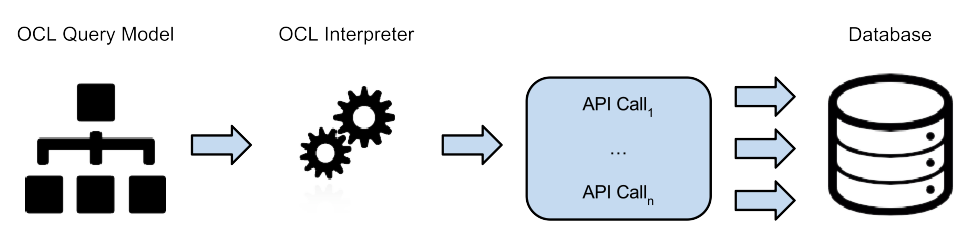
\includegraphics[width=\textwidth]{neoemf-discussion.png}
  \end{center}
	\begin{itemize}
	\item Low-level model handling APIs
	\item Fragmented queries on the database
	\item Many intermediate objects
	\end{itemize}
\end{frame}

\section{Mogwa\"i}

\begin{frame}[c]\frametitle{Motivation}
	\begin{itemize}
	\item Why don't we query directly the database?
	\item Manually writing database-level queries is hard
	\item Need to learn a new query language
	\item Database expertise vs. Modeling expertise
	\item Unknown model representation
	\item Solution: generate them!
	\end{itemize}
	
\end{frame}

\begin{frame}[t]\frametitle{Mogwa\"i: Architecture~\cite{DBLP:conf/rcis/DanielSC16}}
  \begin{center}
    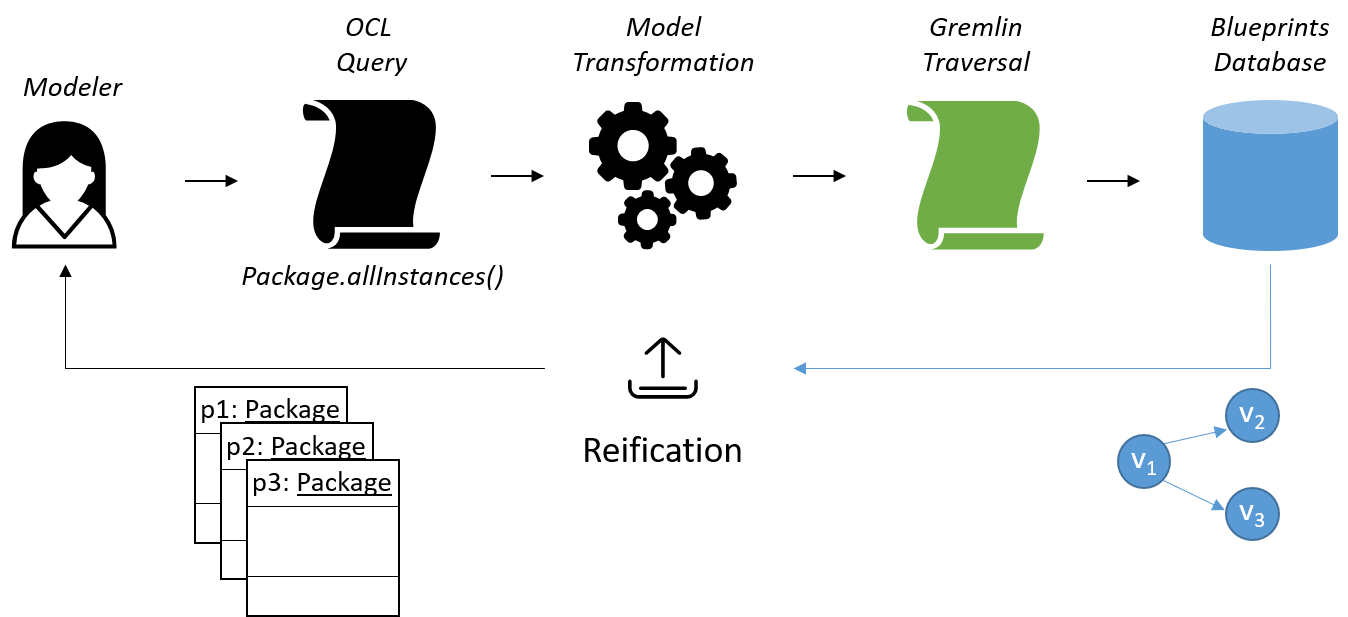
\includegraphics[width=\textwidth]{mogwai-architecture.png}
  \end{center}
	\begin{itemize}
	\item Generate graph database queries from OCL expressions
	\item Bypass modelling framework API
	\item Single execution of the query
	\end{itemize}
	
\end{frame}

\begin{frame}[c]\frametitle{Mogwa\"i: project website}
  \begin{center}
    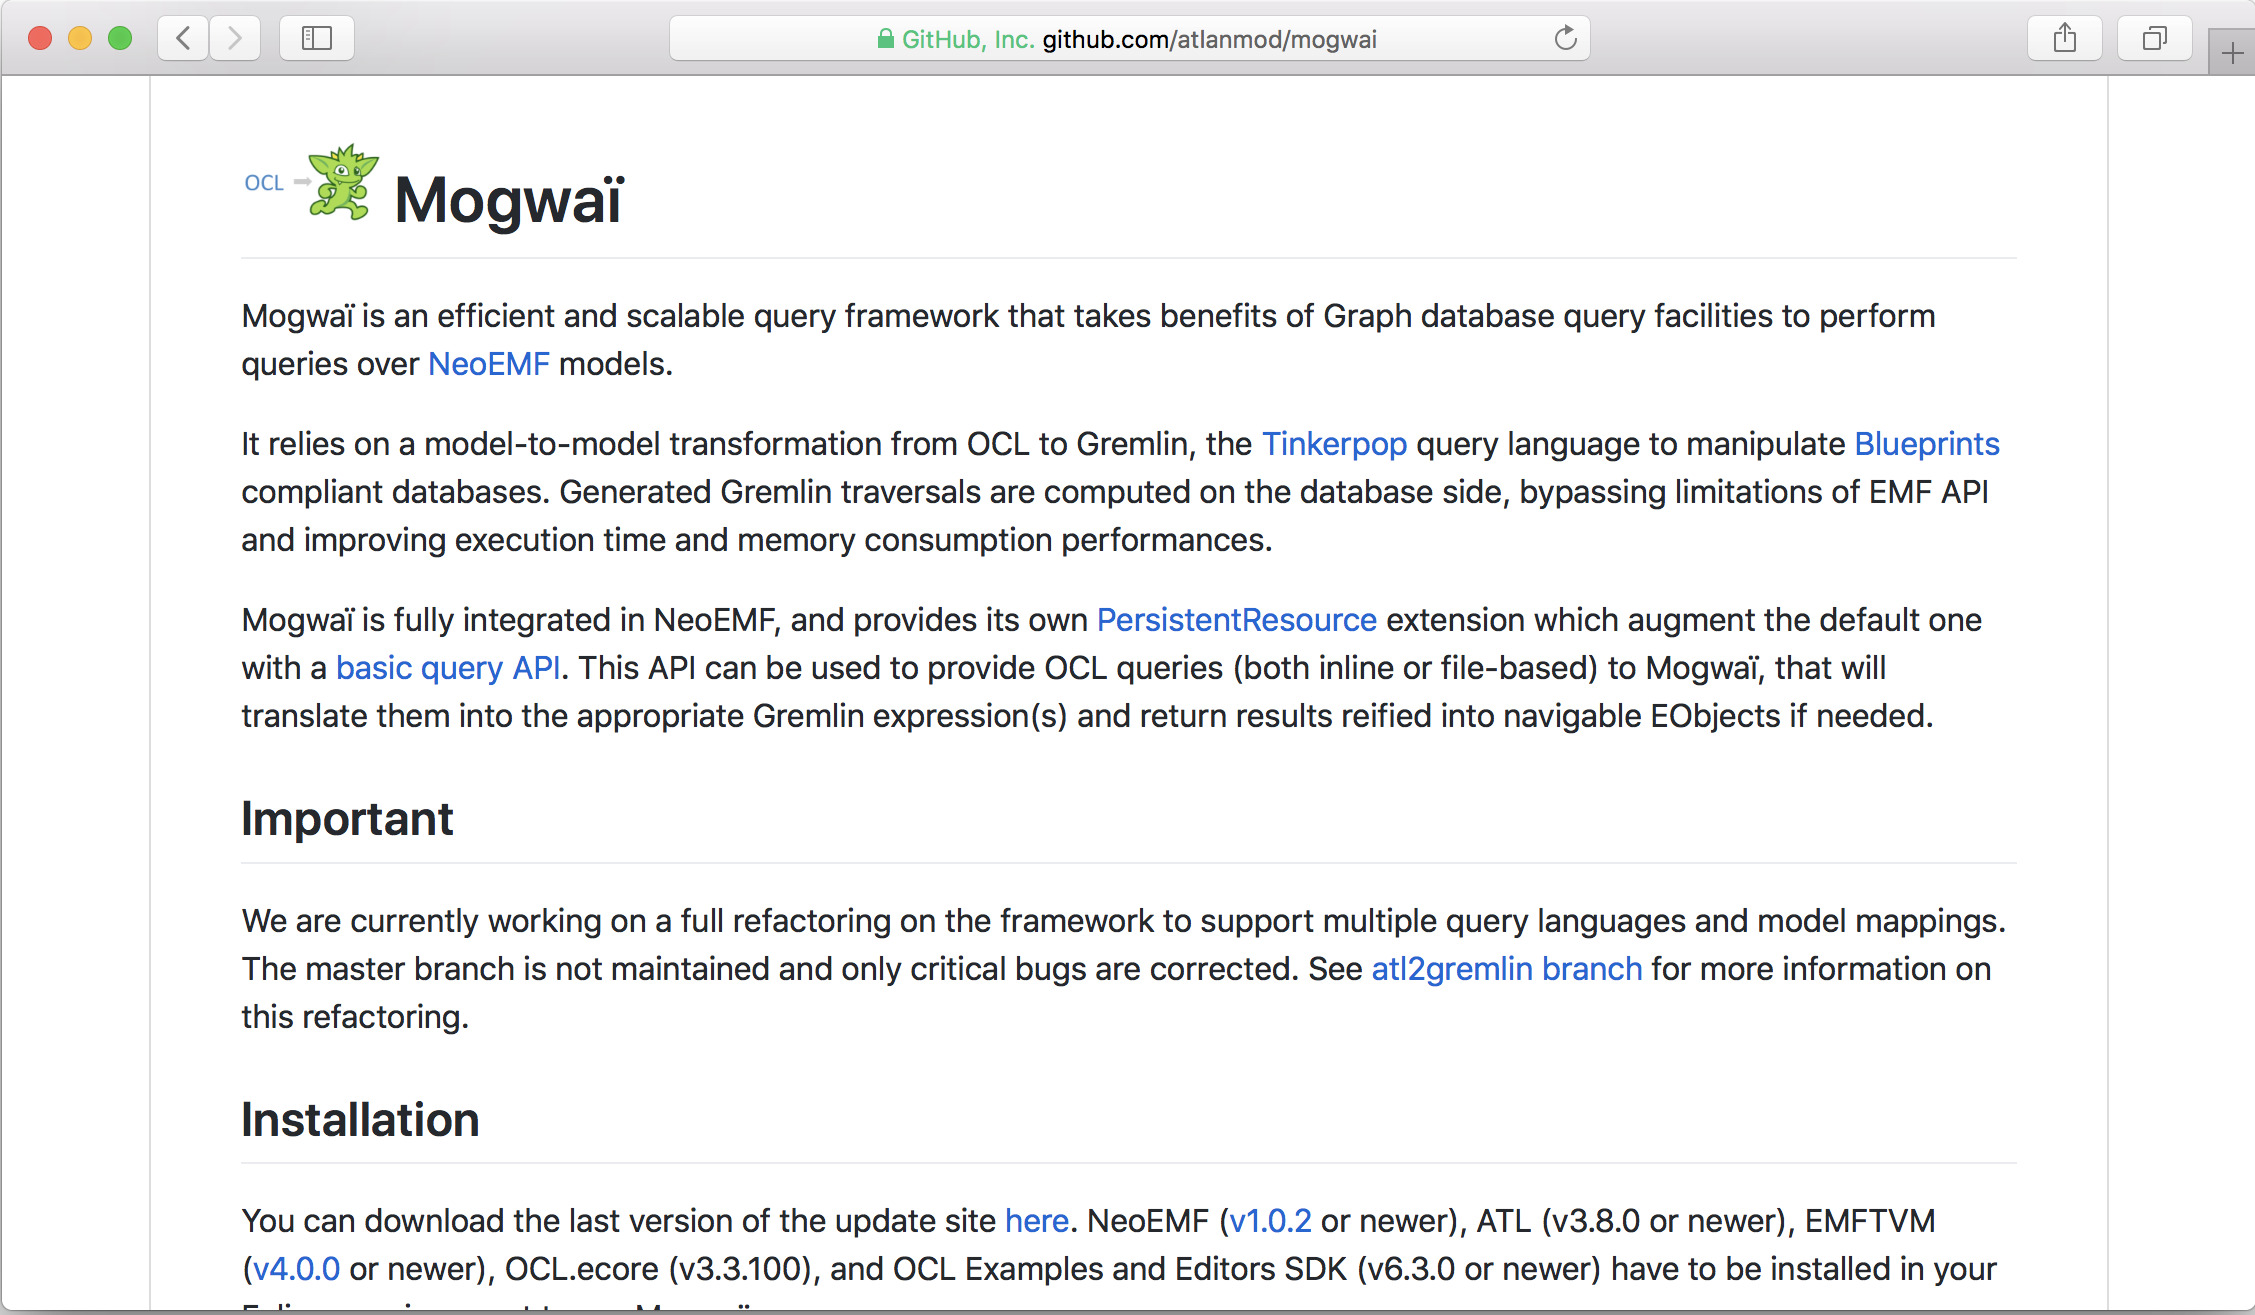
\includegraphics[width=\textwidth]{mogwai-github.png}
  \end{center}
	
  \begin{itemize}
  \item \url{https://github.com/atlanmod/mogwai}
  \item Open source project under the Eclipse Public License 2.0
  \end{itemize}
\end{frame}

\begin{frame}[fragile]\frametitle{Queries are expressed in OCL}
	
	\begin{columns}
		\begin{column}{0.5\textwidth}
	    \begin{figure}[htbp]
		    \centering
			  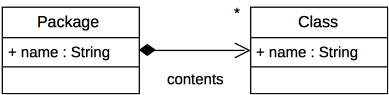
\includegraphics[width=\textwidth]{mogwai-model.png}
		    \caption{Simple Model}
	    \end{figure}
	    \begin{figure}[htbp]
		    \centering
			  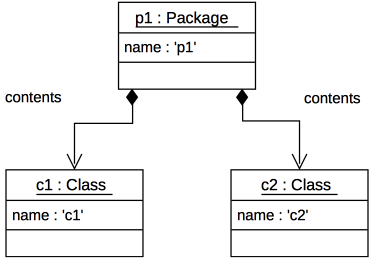
\includegraphics[width=\textwidth]{mogwai-instances.png}
		    \caption{Model Instances}
	    \end{figure}		
		\end{column}
		\begin{column}{0.5\textwidth}
		  \begin{ocl}
        Package.allInstances()  -- returns p1
        p1.contents				-- returns [c1,c2]
        p1.contents->select(e | e.name = 'c1') 
		    -- returns c1
		  \end{ocl}
		\end{column}
	\end{columns}
\end{frame}

\begin{frame}[c]\frametitle{Model Persistence}
	\begin{figure}[htbp]
		\centering
		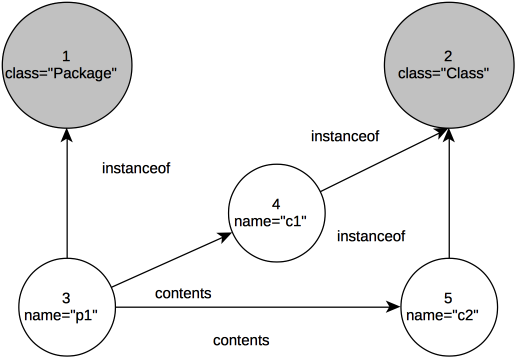
\includegraphics[width=.6\linewidth]{mogwai-graph.png}
		\caption{Model Instances Stored in Neo4j}
	\end{figure}
\end{frame}

\begin{frame}[fragile]\frametitle{Database Queries are expressed in Gremlins}
	\begin{itemize}
	\item Graph traversal DSL
	\item Composed of processing steps
	\item Generic query language for graph databases
	\end{itemize}
	\begin{columns}
		\begin{column}{0.4\textwidth}
			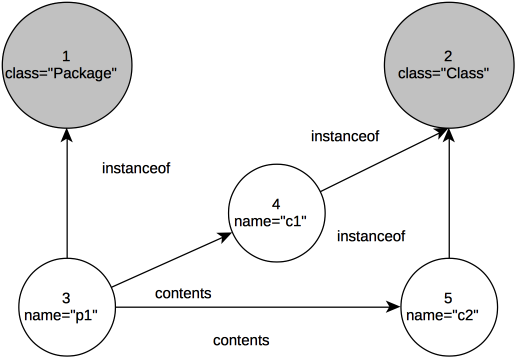
\includegraphics[width=\linewidth]{mogwai-graph.png}
		\end{column}
		\begin{column}{0.6\textwidth}
      \begin{lstlisting}[language=gremlin]
        g.idx(''metaclasses'')[[name:''Package'']]
        .inE(''instanceOf'').outV // v(1)
        g.v(3).outE(''contents'').inV // [v(4),v(5)]
        g.v(3).outE(''contents'').inV
        .filter{it.name = ''c1''} // v(4)
      \end{lstlisting}
		\end{column}
	\end{columns}
	
\end{frame}

\begin{frame}[c]\frametitle{OCL Queries into Gremlin Traversals Translation}
	\begin{itemize}
	\item Map OCL expressions to Gremlin steps
	\item Merge created steps into a (several) traversal(s)]
	\end{itemize}
  \begin{center}
    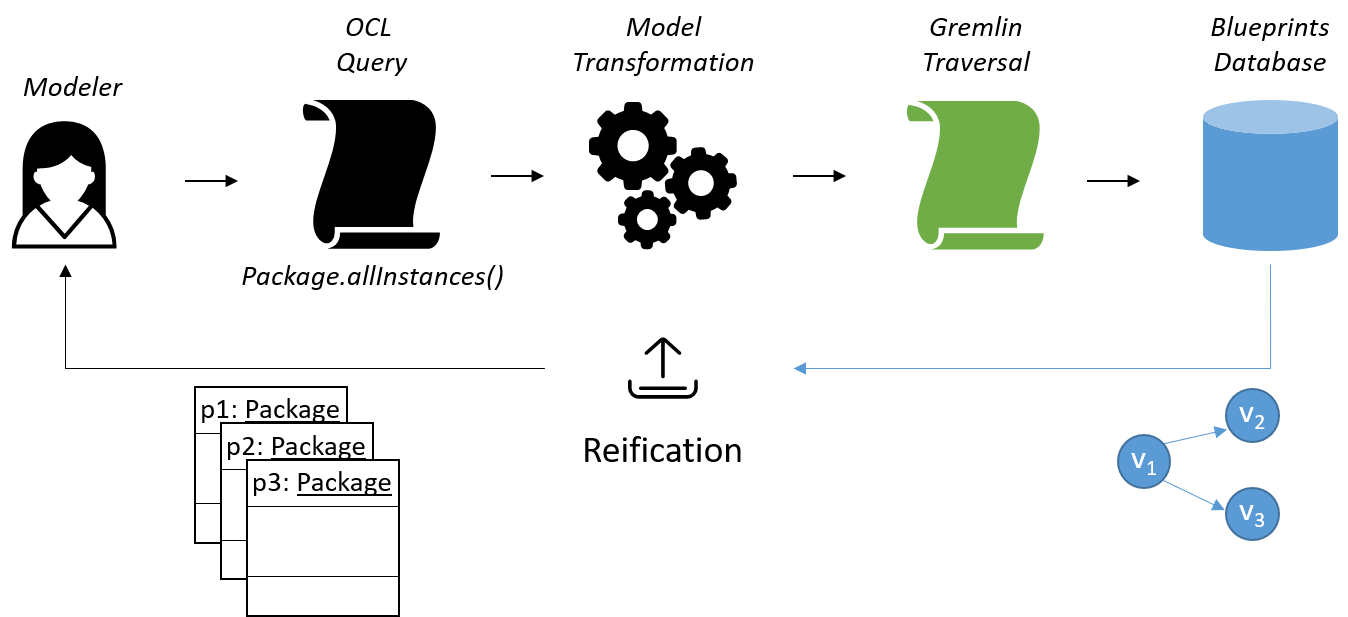
\includegraphics[width=\textwidth]{mogwai-architecture.png}
  \end{center}	
\end{frame}

\begin{frame}[c]\frametitle{OCL Expressions to Gremlin Steps Mapping}
	\begin{columns}
		\begin{column}{0.5\textwidth}
      \begin{center}
        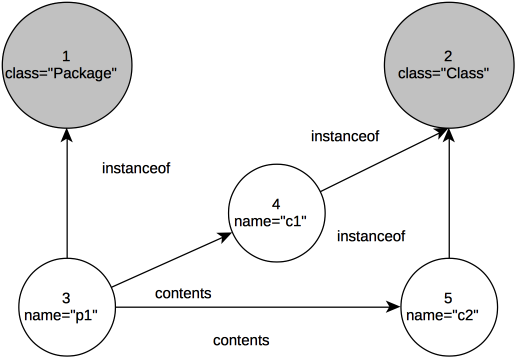
\includegraphics[width=\textwidth]{mogwai-graph.png}
      \end{center}			
		\end{column}
		\begin{column}{0.5\textwidth}
      \begin{center}
        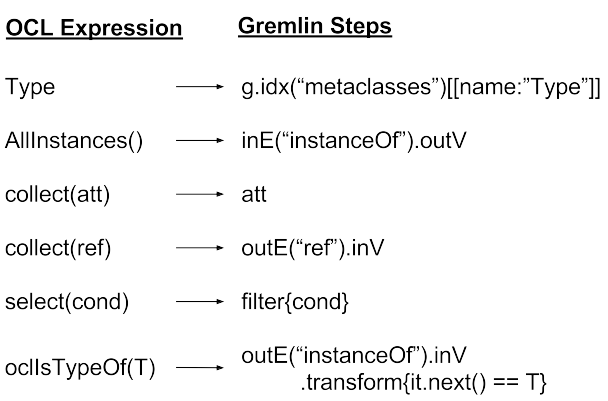
\includegraphics[width=\textwidth]{mogwai-mapping.png}
      \end{center}			
		\end{column}
	\end{columns}
\end{frame}

\begin{frame}[c]\frametitle{Merge created steps into a traversal}
  \begin{center}
    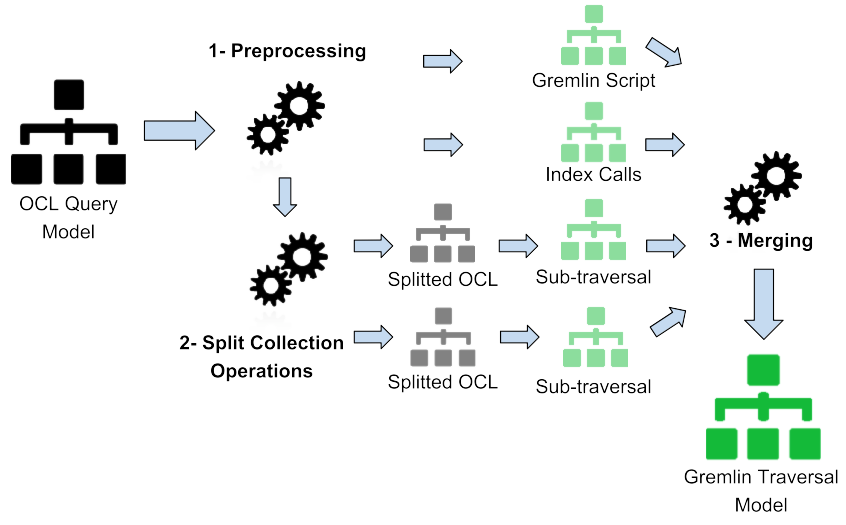
\includegraphics[width=\textwidth]{mogwai-transformation.png}
  \end{center}
\end{frame}

\begin{frame}[c]\frametitle{OCL Transformation Example}
  \begin{center}
    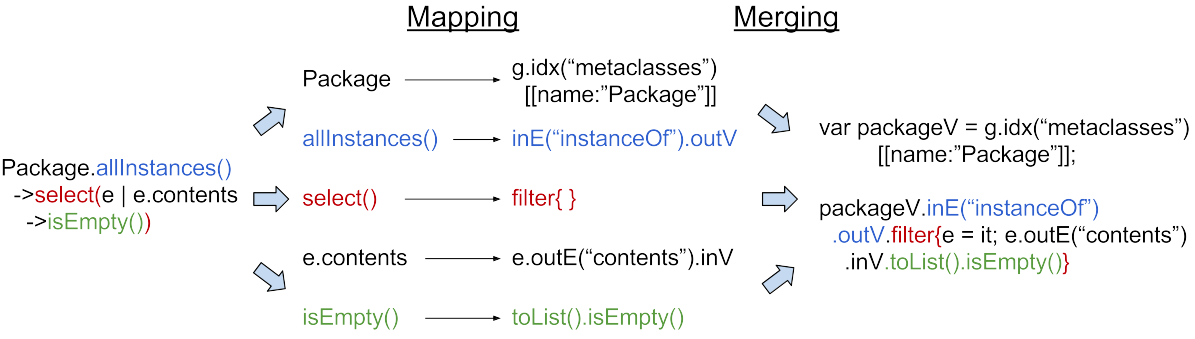
\includegraphics[width=\textwidth]{mogwai-ocl-transformation.png}
  \end{center}	
\end{frame}

\begin{frame}[c]\frametitle{Query generation and execution}
	
	\begin{itemize}
	\item Delegates query computation to the database
	\item Returns graph elements to the persistence layer
	\end{itemize}
	
  \begin{center}
    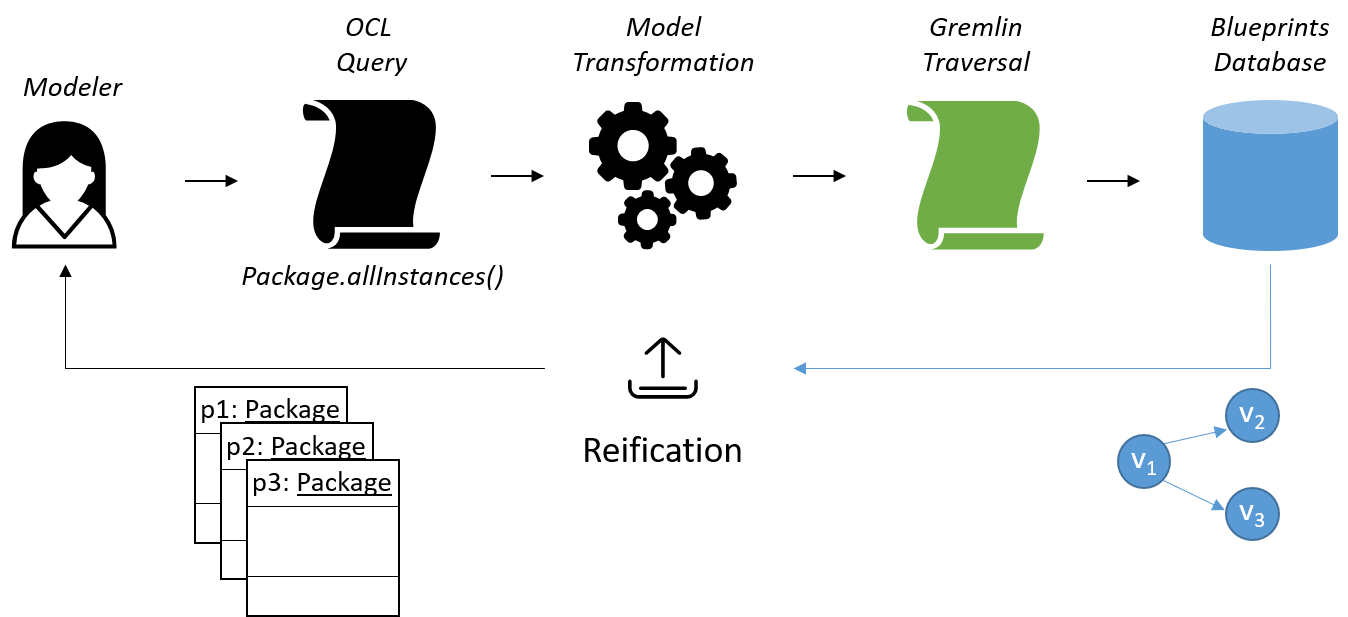
\includegraphics[width=\textwidth]{mogwai-architecture.png}
  \end{center}
	
\end{frame}

\begin{frame}[standout]
  Demo time!

  Let's query a Java model and find singletons.
\end{frame}

\begin{frame}[c]\frametitle{Benchmark Results}

  \begin{itemize}
	\item Model containing 2 million elements
	\item Up to 20 times faster than other query approaches
	\item Consume up to 75 times less memory
  \end{itemize}
  \begin{columns}
	  \begin{column}{0.5\textwidth}
	    \begin{center}
	      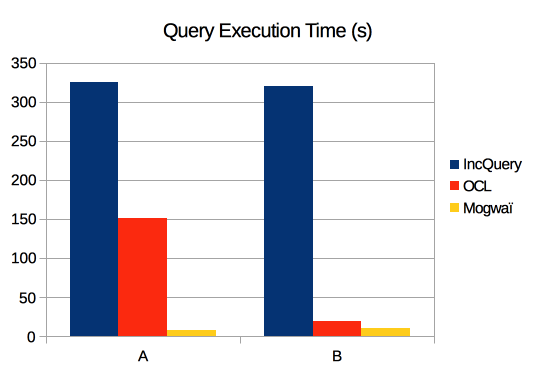
\includegraphics[width=\textwidth]{mogwai-benchmark-cpu.png}
	    \end{center}
	  \end{column}
	  \begin{column}{0.5\textwidth}
	    \begin{center}
	      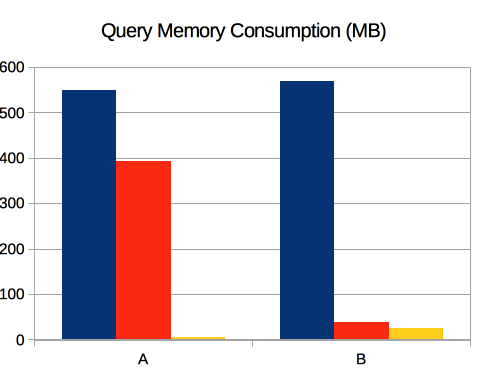
\includegraphics[width=\textwidth]{mogwai-benchmark-memory.png}
	    \end{center}
	  \end{column}
  \end{columns}

\end{frame}

\begin{frame}[c]\frametitle{Conclusion}
	\begin{block}{Model Persistence Frameworks}
	  \begin{itemize}
		\item Not designed to compute model queries efficiently
		\item Writing manually database-level queries is hard
	  \end{itemize}
	\end{block}

  \begin{block}{Mogwaï}
		\begin{itemize}
		\item Translates OCL queries into Gremlin traversals
		\item Positive results
		\item Not adapted to small models
		\item Needs to be integrated
	  \end{itemize}
  \end{block}
\end{frame}

\pgfset{/metropolis/inner/sectionpage/.cd, none}
\section{Wrap-up}

\begin{frame}[allowframebreaks]{References}
  \bibliography{../bibliography}
  \bibliographystyle{alpha}
\end{frame}

\end{document}
